\chapter{Simulating Cyber-Physical Systems in the Virtual-World (10)}
% Describe what better CPS tools would provide - environmental simulation, trained environment models, virtual environments, cross-environment simulation

Testing and understanding how the environment interacts with a sensor network and vice-versa relies on placing the devices in the target environment and waiting for/creating the desired phenomena to interact with the network. Performing tests in the real-world is time-consuming, costly and often impracticle. Carrying out tests utilising human mobility also poses difficulties. Phenomena can include events such as movement of devices/objects, passive or active interaction with people (pressing buttons, triggering motion sensors), or other sensor events. Performing test deployments can be expensive, time-consuming and difficult.


% In this chapter we present and evaluate a novel approach to this problem, integrating a freely available high-performance 3D video game engine (Unreal Engine 4) with an existing sensor network simulation platform (Cooja), creating an end-to-end simulation solution for realistic testing of sensor networks in their target environments. By integrating a 3D game engine, we are introducing sensor network simulations into virtual reality with a real-time and dynamic virtual world, utilising the game engine's realistic physics, lighting and artificially intelligent people and crowds to influence and test the deployed sensor network.

% In the following section we describe in detail our novel 3D simulation platform, Ard\'{a}n, discussing the various features and tools it provides. Section 2 discusses the requirements which we believe to be vital for 3D simulation platform development. Section 3 describes the design and architecture of Ard\'{a}n, followed by an example case study for testing and deployment in section 4. We subsequently present a performance evaluation and discuss the challenges involved in developing the Ard\'{a}n platform, in sections 5 and 6 respectively.
\section{Problem} % (fold)
\label{sec:problem}
Discuss how existing tools/simulators don't focus on simulating the environment, instead focussing on accurate hardware/software simulation. 
Existing approaches for testing CPS focus heavily on accurately simulating devices, the network and power consumption, with great success \cite{cooja, tossim}.
These tools and techniques don't support reliably, comprehensively and dynamically testing these devices in the context of their target environment and the phenomena which may occur within it. Typically, the environment fed into simulations using recorded sensor traces or fabricated based on a developers model and needs. These traces:
\begin{itemize}
  \item static - recorded traces are taken from fixed positions, can be modified but is time consuming and un-reliable
  \item reliability - fabricated traces are based on a developers model of an environment and may not accurately represent it or all of it.
  \item comprehensive - traces are time consuming to create and must be created ahead of time
\end{itemize}

performed using recorded or designed sensor trace data. This approach can be inaccurate, unrealistic and is restricted to what was recorded.

% section problem (end)
\section{Design}
\label{sec:Design}

The WSN simulator (Cooja), performs all application and network simulation for the co-simulation and is configured with a set of nodes with their 3D location and application code to run. As the application code is run in real-time, any sensor- or actuator-based hardware requests, such as sensor reads and actuator commands, are forwarded to the 3D game engine to be performed in the virtual environment.

Within the Unreal Engine we modeled a 3D environment and created a several components to support deploying virtual sensor networks, including device and sensor 3D models, hardware abstractions for the virtual sensors and actuators to sense the virtual world and report back to the simulator over the network bus. Similarly within the Cooja simulator we have modified the simulated hardware to communicate to our virtual hardware in the Unreal Engine.

Using Cooja, developers are able to write code once and both test in Ard\'{a}n and deploy in the real-world on the Contiki or TinyOS platform, removing difficulties associated with translating between test and deployment platforms. Using the open architecture, support for additional tools and simulation platforms can also be added, expanding the possibilities and improving the fidelity of simulations.

\section{Phenomena-on-demand} % (fold)
\label{sec:phenomena_on_demand}
Unlike existing approaches which utilise purely trace-fed and scripted approaches which are static and difficult to modify, this simulator enables dynamic phenomena generation based on the user input or scripted behaviour. 
By taking direct control of devices or people within the environment, developers can iteract with and modify the simulation directly and observe how the dynamic simulation responds. This differs to trace-fed alternatives which require developers to manually change the input to sensors based on how they believe the environment has changed. 

For example, two sensors are placed within a school corridor to detect the pace of people walking past; the sensors communicate and calculate the walker's pace, displaying a red light to people running. In a trace-fed scenario, developers script sensor detection inputs to the two nodes. Developers may generate a test case for different speed walkers or multiple walkers. For each test case, the developers need to manually calculate and modify each trace-feed for each sensor individually. For our approach, developers need only change the speed of a person walking and observe the effects on the system. This approach provides a much more intuitive and scalable solution to testing with large numbers of devices and as the number of input sensors increase, in which trace-fed solutions become unmaintainable.  
% section phenomena_on_demand (end)

\section{Mobility} % (fold)
\label{sec:mobility}

% section mobility (end)
\section{Communication} % (fold)
\label{sec:communication}

% section communication (end)
\section{Synchronisation} % (fold)
\label{sec:synchronisation}

% section synchronisation (end)



\section{Forward Time Control} % (fold)
\label{sec:time_control}

\section{Distribution} % (fold)
\label{sec:distribution}

% section distribution (end)

\section{Case Study}
\label{sec:Case Study: Corridor}

The purpose of the following case study is to demonstrate what development of a non-trivial CPS application is like using Ard\'{a}n, and how it enables developers to test and visualise different scenarios, by simply adding or moving devices or people in the simulation.

The case study focuses on controlling the lighting within a modern day office corridor, with the goal of striking a balance between energy efficiency, effective lighting and user comfort. The ideal corridor lighting scheme should provide a pleasant lighting scheme for users of the corridor, able to adjust based on ambient light levels, gradually illuminating as they progress through it, whilst also ensuring energy is minimised by turning off or reducing the brightness of unused or infrequently used parts of the corridor.

Thus, this provides an interesting and non-trivial task, due to the many ways in which the corridor can be entered/exited or moved around within in; people can enter from the beginning, end or from a room; people can move down the length of the corridor or directly from room to room; people often also stop in the corridor, spending time talking or waiting. Similarly, understanding the ideal number and placement for devices and sensors, and how it affects applications, such as power, reliability, robustness etc. Hence, providing effective lighting schemes can prove difficult to analyse and reason without rigorous testing.

The rest of this section will demonstrate and discuss the use of Ard\'{a}n to design, analyse and test for our target environment, the corridor, highlighting the features and benefits that the tool provides.


\begin{figure*}[t]
  \centering
  \subfloat[Over-the-shoulder view]{
    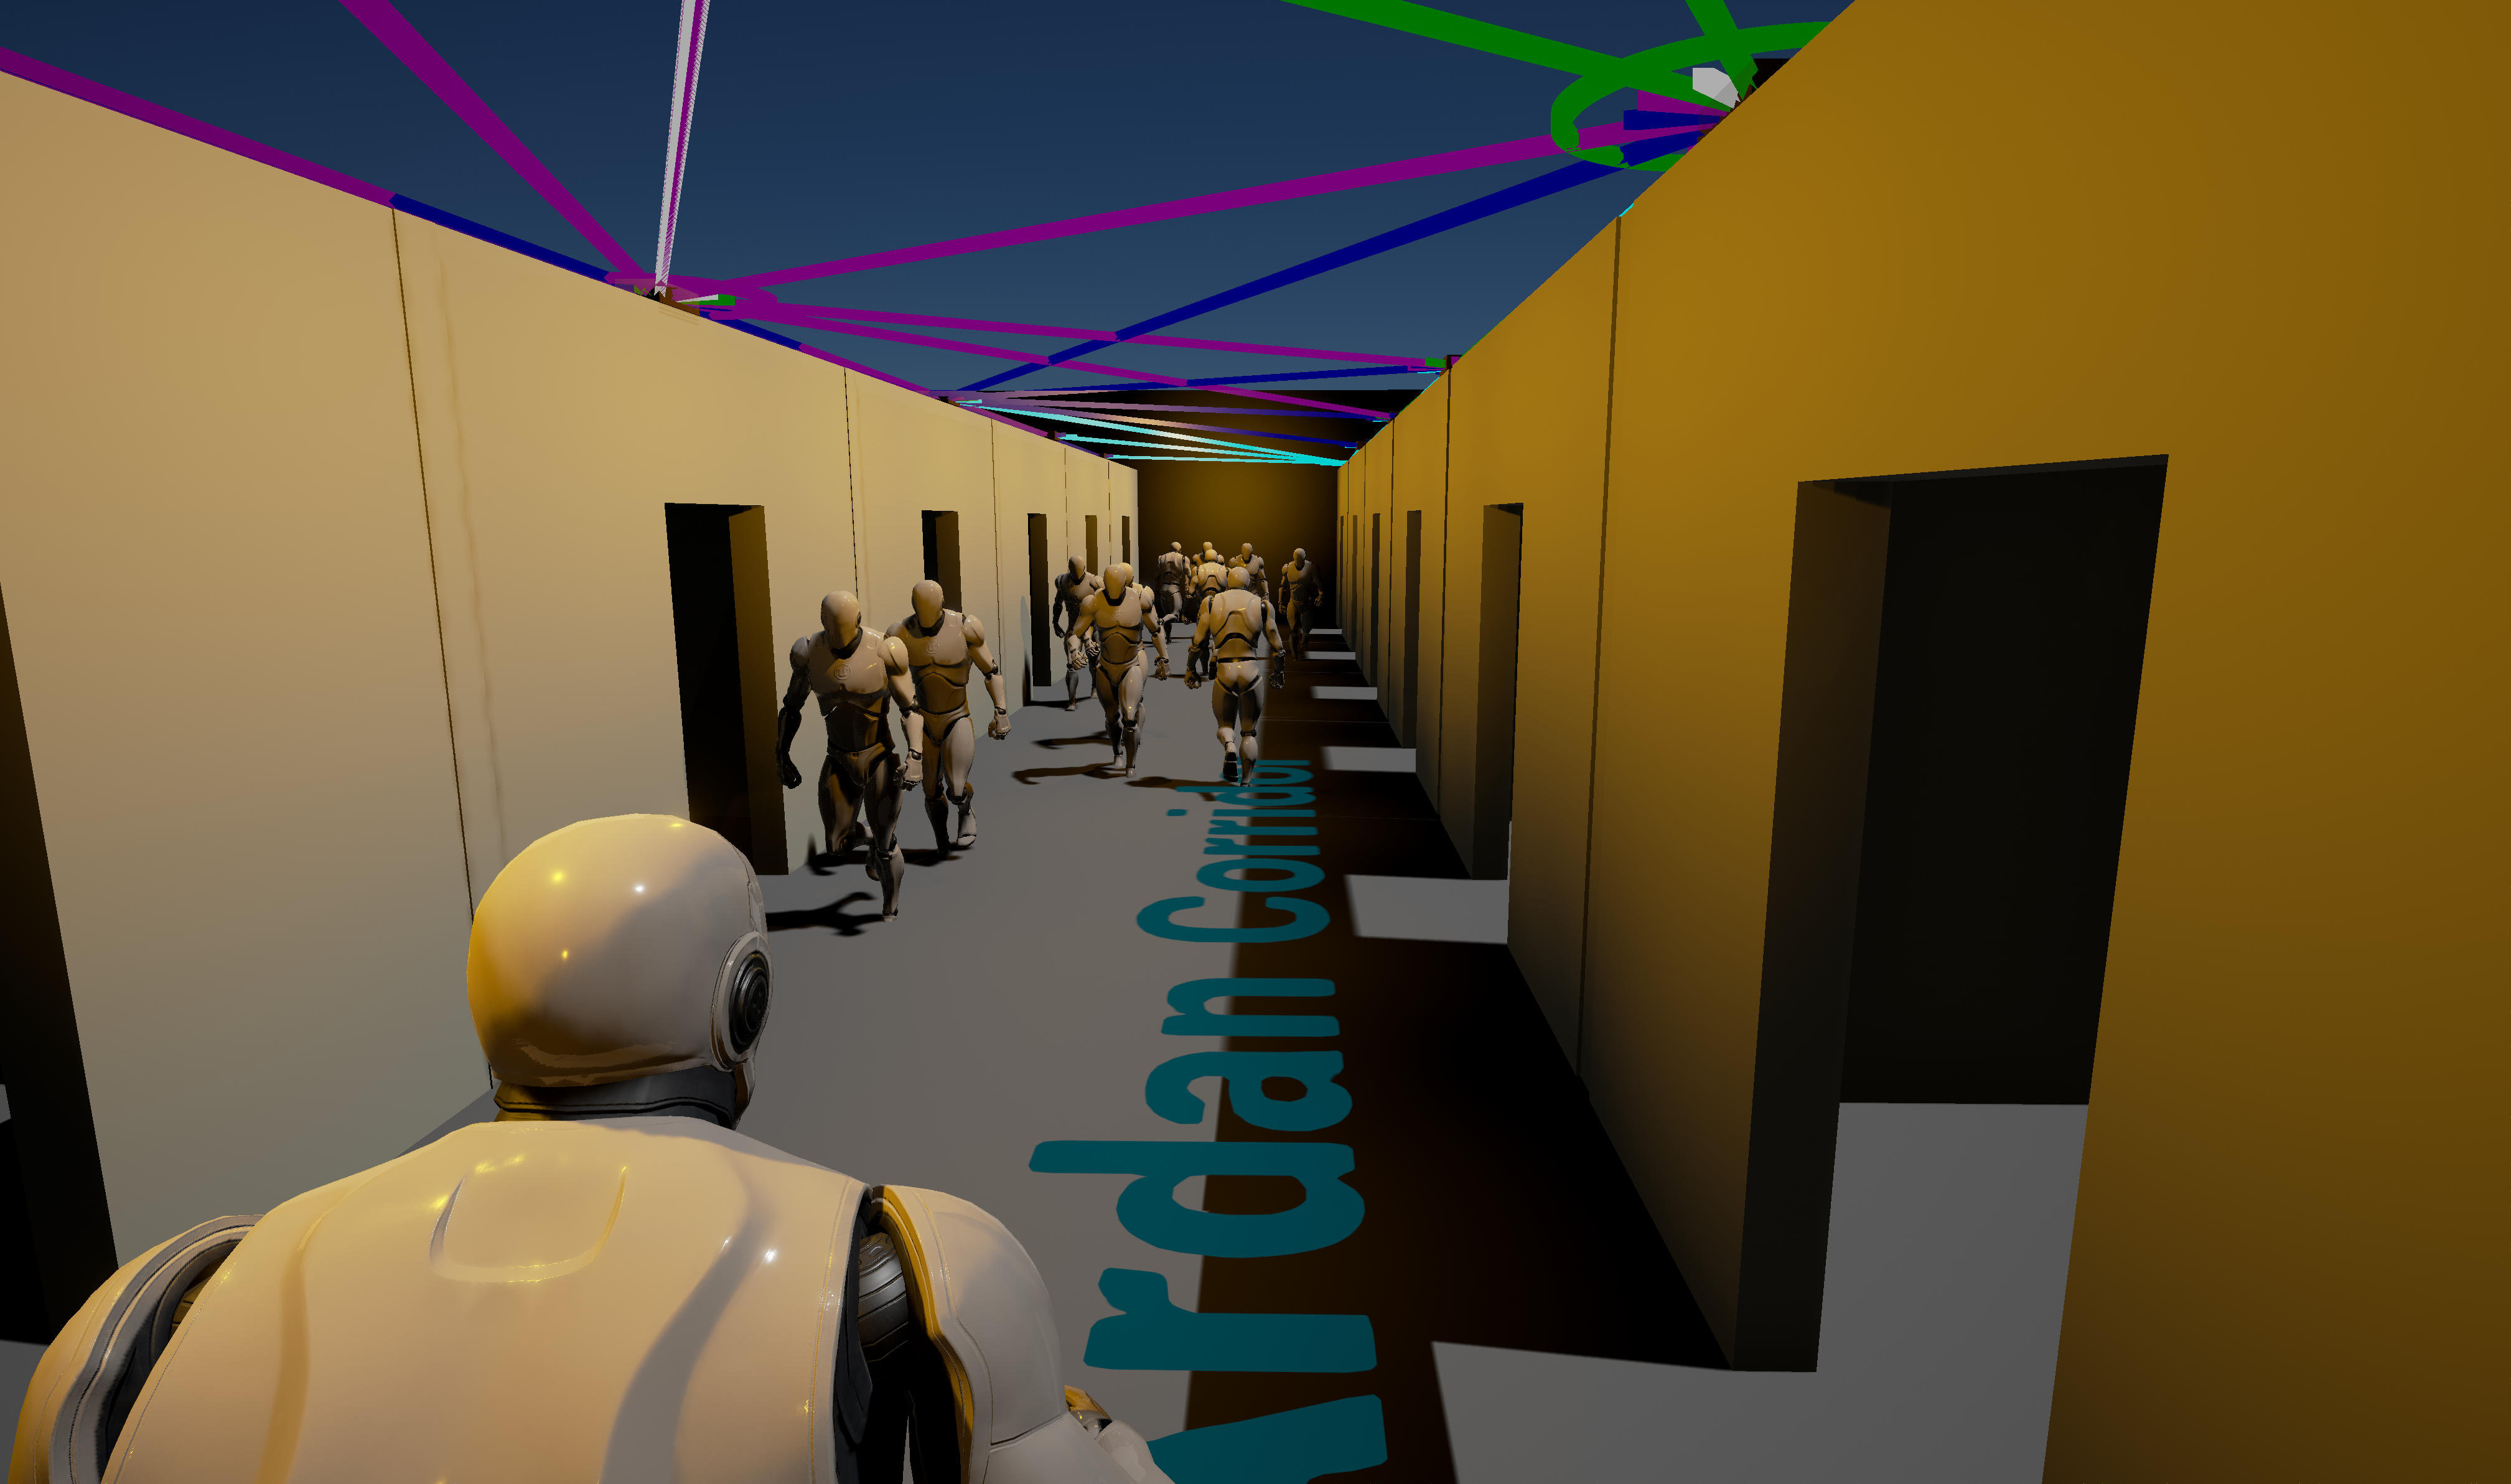
\includegraphics[height=2.6cm]{imgs/OverShoulder.jpg}
    \label{fig:birds_view}
  }
  \subfloat[Birds-eye view]{
    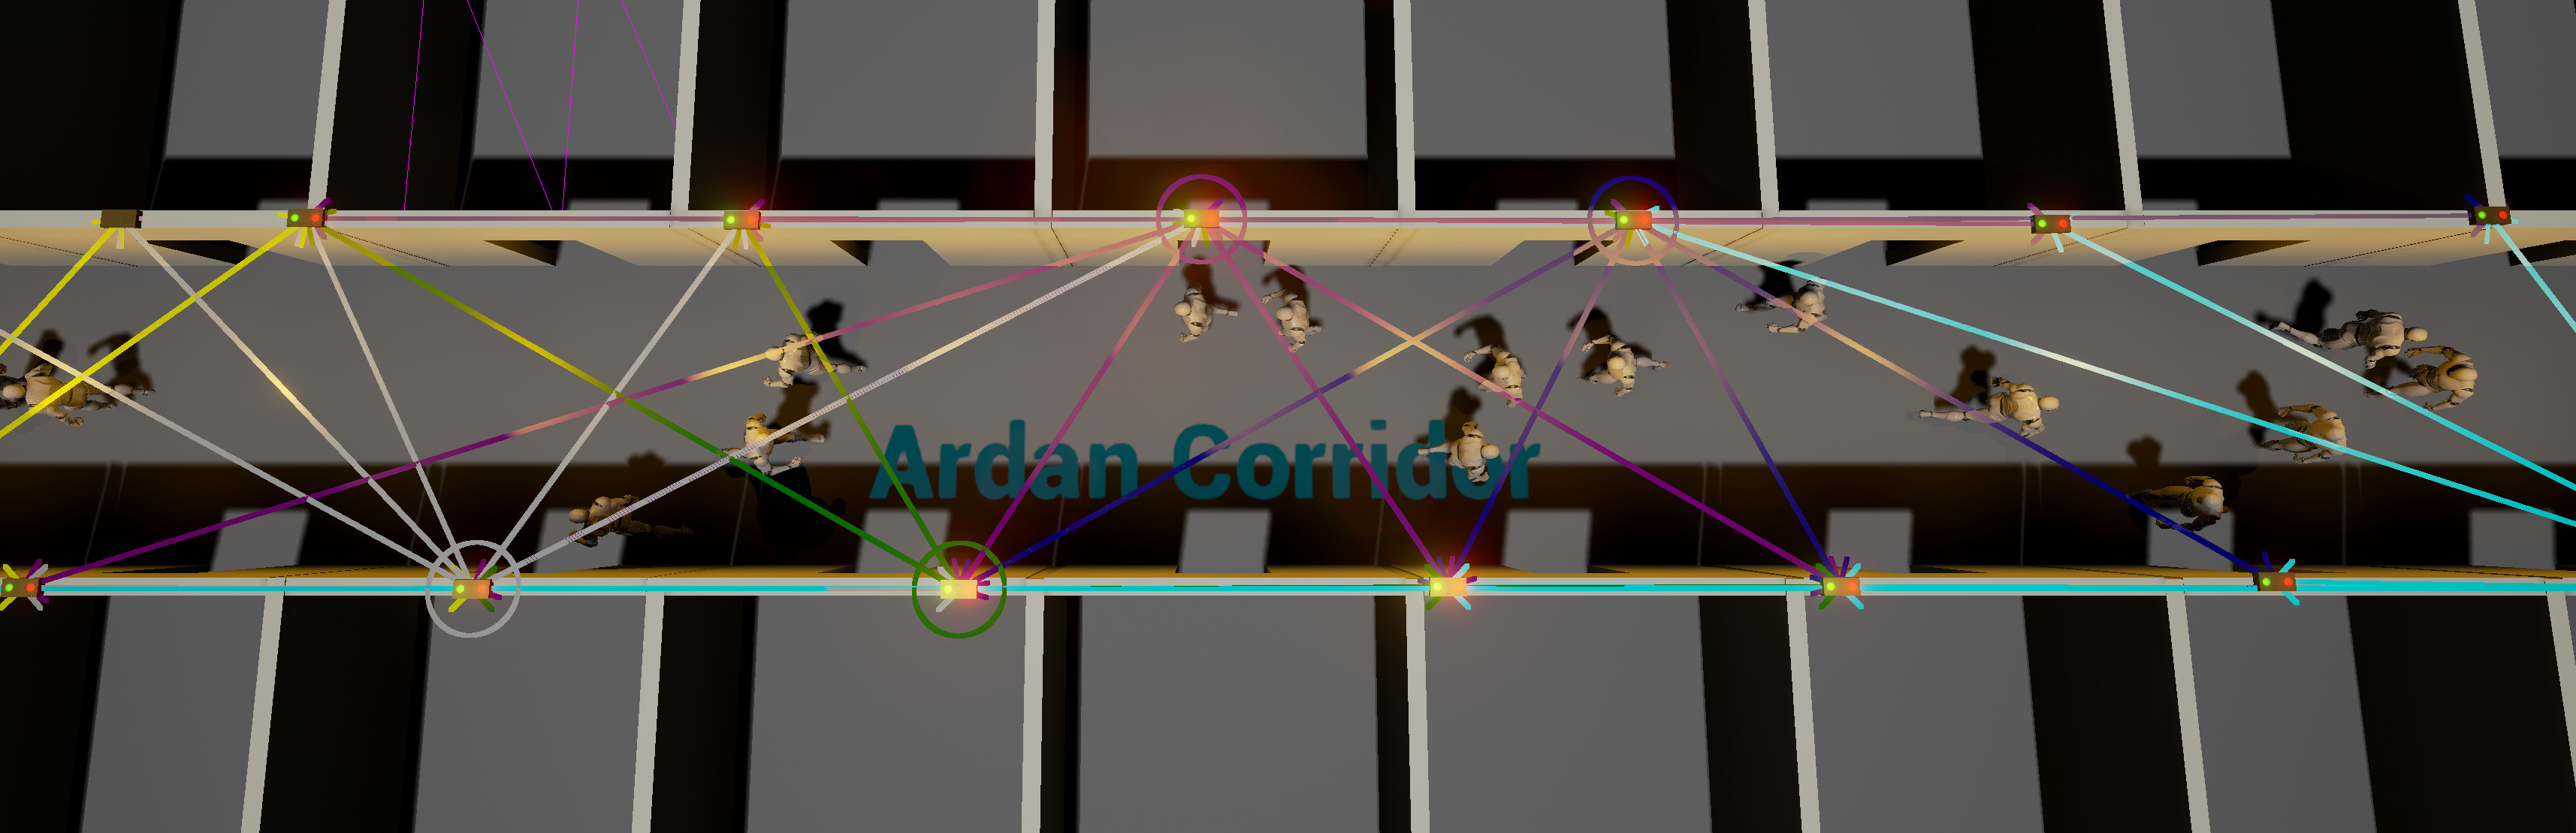
\includegraphics[height=2.6cm]{imgs/BirdsEye2.jpg}
    \label{fig:shoulder_view}
  }
  \subfloat[Camera view]{
    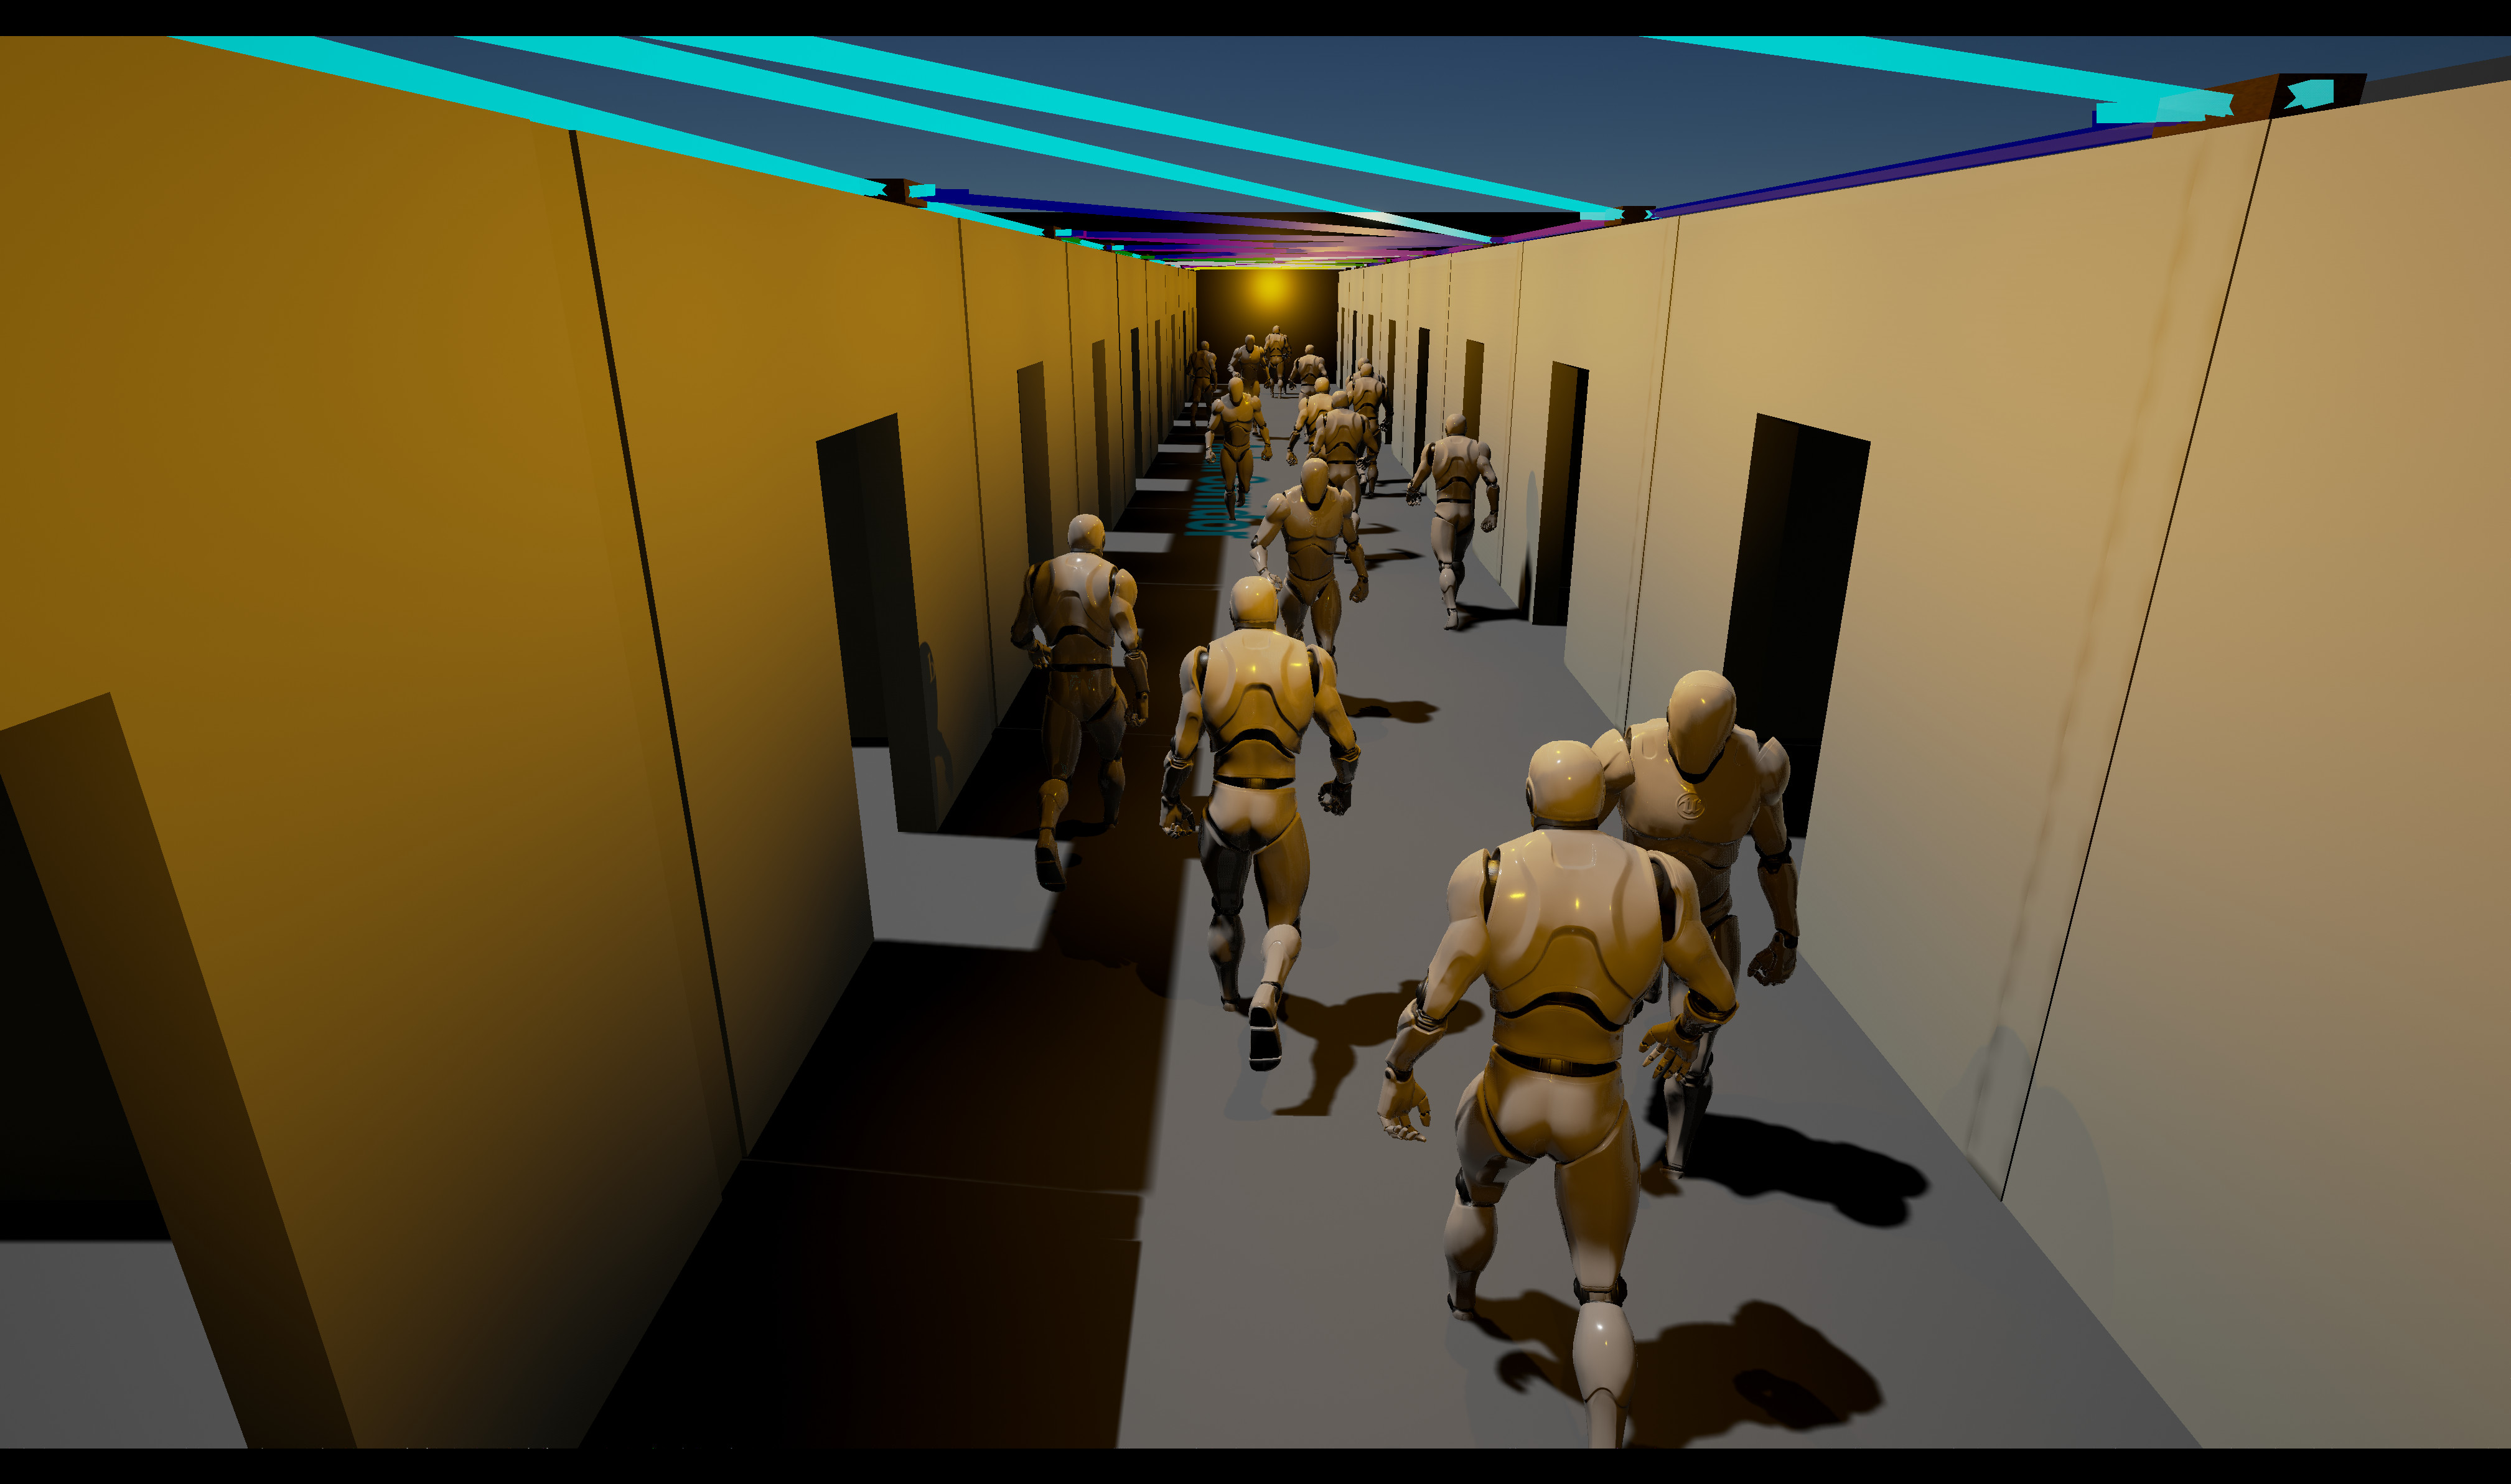
\includegraphics[height=2.6cm]{imgs/Camera.jpg}
    \label{fig:camera1_view}
  }
  \caption{15 people walking up and down the virtual corridor, triggering motion sensors}
  \label{fig:views}
\end{figure*}


\subsection{Corridor Design}
\label{sub:Constructing the corridor}
We created a virtual corridor based on a real corridor within our building, measuring 20x 1.5 meters, with 5 doors spaced evenly on either side. Along the corridor we placed 15 nodes with lights and conical motion sensors attached to the ceiling facing the floor directly below, shown in figure \ref{fig:corridor_layout}.

To construct the corridor, we used pre-existing models for walls, doorways and lights, making it quick to build or modify. In addition to these, we've created several new models for nodes and a variety of sensors, which can be composed together to create different sensing devices. A drag-and-drop interface is used to place nodes within the newly built 3D environment. The node model is based on a small box with 3 coloured lights, representing the typical LED outputs available on devices, such as the TelosB mote.

The next step was to create the nodes in the Cooja simulator, compiling and loading node application code. Using the IDs Cooja assigns to these nodes, the virtual representations were assigned matching IDs. This is especially important when certain applications are loaded on particular nodes, or when node IDs are used programmatically e.g., for location, routing or ordering.

\subsection{Lighting Algorithm}
\label{sub:Lighting Algorithm}
For demonstrative purposes, we developed a basic lighting algorithm based on our needs described previously. The algorithm, shown as pseudo code in figure \ref{fig:algorithm}, and developed further in figure \ref{fig:algorithm2}, waits for a motion detection event before illuminating its light for 5 seconds and notifying its closest neighbours. If it receives a message from a neighbour, it checks that it's adjacent, before illuminating its light for 3 seconds. The second variation attempts to build upon this algorithm, improving the lighting efficiency, using the simulator to test and experiment.

Using this as a base, we expect to test and iterate the algorithm based on our findings from our ``What if?'' scenarios.
\begin{figure}
\begin{verbatim}
  wait (event):
    if event == network:
      if msg.src + 1 == me or msg.src - 1 == me:
        turn_on_light(3000)
    if event == PIR:
      turn_on_light(5000)
      alert_neighbours()
\end{verbatim}
\caption{Lighting algorithm psuedo-code}
\label{fig:algorithm}
\end{figure}
\begin{figure}
\begin{verbatim}
  wait (event):
    if event == NETWORK and msg.dst == me:
      turn_on_light(5000)
      if msg.src + 1 == me:
        dir = FORWARD
      else if msg.src - 1 == me:
        dir = BACKWARD

    if event == PIR:
      turn_on_light(5000)
      if dir == FORWARD:
        alert_neighbour(FORWARD)
      else dir == BACKWARD:
        alert_neighbour(BACKWARD)
\end{verbatim}
\caption{Lighting algorithm psuedo-code with direction}
\label{fig:algorithm2}
\end{figure}



\subsection{``What if?'' scenarios}
\label{sub:Creating test scenarios}
When testing CPS deployments, ``what if'' questions about how the system will perform will naturally arise, such as ``what if we move or increase/decrease the number of nodes?'', or ``what if there are multiple people?'', or ``what if we place sensors differently or use more/less sensitive ones?''. Being able to quickly test and understand what happens to a system in these different scenarios is key to improving its reliability and efficiency.

In order to test our lighting application we devised several test scenarios to test both basic and complex situations for which we expect the system to perform correctly with; the complexity of a scenario increases as the number of agents in the scene increases and the pattern of movement changes from simple start to end directions, thus becoming more difficult to visualise and debug conceptually.

Using Ard\'{a}n, we are able to directly control a person in the virtual space, directing them down the corridor and observing, from multiple angles, the lighting algorithm reacting to their presence. This provides ultimate control in creating dynamic and new test scenarios, allowing developers to run around without any of the drawbacks of performing the same tests in real-life, such as fatigue, health and safety and time.

We also have the ability to adjust the number and placement of nodes within the environment, enabling us to test different configurations and determine which works best and fits our requirements.

Unlike the real world, using Ard\'{a}n we are able to pause the entire simulation, giving developers more time to understand the state of the network and virtual world at a particular point in time, before stepping through or continuing the simulation. On top of this, we are also able to change our view point between the cameras placed in the virtual world or move freely about within it to fully capture and understand the state of the environment whilst the simulation and world are paused, otherwise not possible in recorded videos of a real-world deployment.

Tests:
\begin{enumerate}
  \item One person
    \begin{itemize}
      \item Walks from end to end
      \item Walks from room to room
      \item Walks, stops, walks opposite direction
    \end{itemize}
  \item Multiple people
  \begin{itemize}
    \item Two agents walk from opposite ends
    \item Multiple agents walk in different patterns
  \end{itemize}
  \item Number and Placement of nodes
  \begin{itemize}
    \item 6 nodes, evenly spaced
    \item 6 nodes, with additional sensors placed facing doors
    \item 12 nodes, evenly spaced
  \end{itemize}
\end{enumerate}



\section{Evaluation}
To prove useful for a developer our system needs to scale to support large networks whilst ensuring synchronised behaviour at real-time or faster. To demonstrate the scalability of Ard\'{a}n, we designed a case study based on managing automated lighting in a typical office corridor, illustrated in figure \ref{fig:views}. Within the corridor we placed the sensor nodes and motions sensors. As people walk through a motion sensor, the relevant device is triggered and turns on its light before notifying its neighbours. When neighbours receive a notification they too turn on, providing a path of light illuminating around the walker. This task provides a non-trivial challenge for designing and testing applications that can deal with various scenarios that could occur, including multiple people walking in different directions, entering/exiting for different areas and people stopping/loitering.

The tests were run on the following spec machine: Xeon E5 1650 6Core with HT, 16GB RAM, 256GB SSD and a sufficiently powerful (MSI GeForce GTX 970) graphics card to support the game engine, otherwise, slow response times between the simulator and 3D game engine would cause the simulation to stall and drop below real-time performance.

\subsection{Co-simulator Performance} % (fold)
\label{sub:co_simulator_performance}

% subsection co_simulator_performance (end)
The results in figure \ref{fig:simulator_scalability} show that Ard\'{a}n can support up to 200 sensor nodes running at real-time with the simulator staying reliably synchronised with the game engine. Beyond this, the simulator performance degrades quickly and synchronisation is lost.

\begin{figure}[ht]
  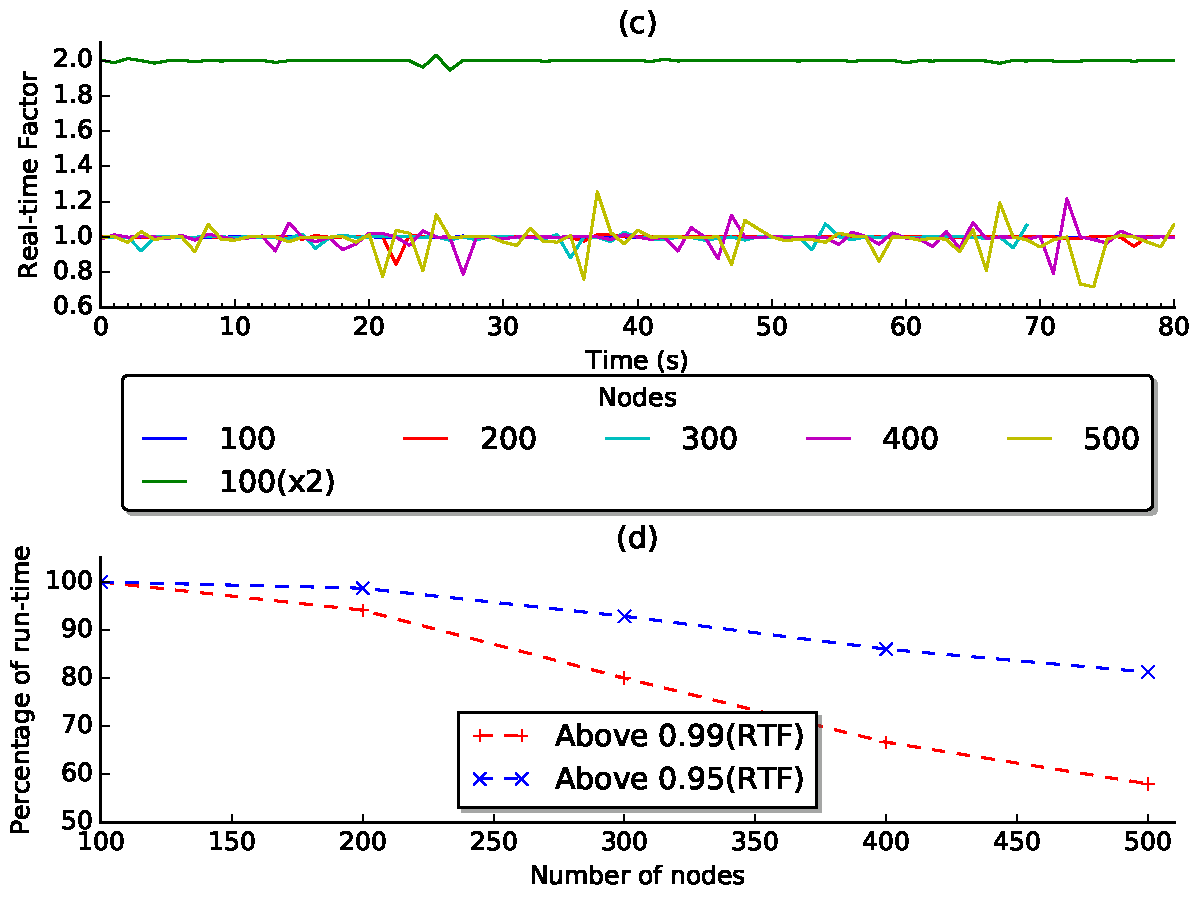
\includegraphics[width=0.5\textwidth]{plots/plot2.pdf}
  \caption{Figure (a) shows how the simulator speed fluctuates over time. Figure (b) shows the percentage of the total run time which the simulation maintains above 99\% and 95\% of its target speed.}
  \label{fig:simulator_scalability}
\end{figure}

Extending further, we also performed tests on running Ard\'{a}n at faster than real-time, at 200\% speed. In this mode, the game engine and its physics engine match the speed of the simulator, resulting in all activity increasing in speed, as opposed to simply increasing the walking speed of individuals. The results in figure \ref{fig:simulator_scalability} show that roughly half the number of nodes can be simulated in time with the game engine, with little fluctuation.

\subsection{Faster-than-real-time Performance} % (fold)
\label{sub:faster_than_real_time_performance}

% subsection faster_than_real_time_performance (end)

% \section{Requirements}
% \label{sec:Requirements}
% Define the list of key requirements described in workshop paper.

% \section{Framework} % (fold)
% \label{sec:framework}

% \subsection{CPS Simulation} % (fold)
% \label{sub:cps_simulation}

% \subsection{Virtual World Simulation} % (fold)
% \label{sub:virtual_world_simulation}
% % subsection virtual_world_simulation (end)
% % subsection cps_simulation (end)

% \subsection{Communication Model} % (fold)
% \label{sub:communication_model}
% % subsection communication_model (end)

% \subsection{Time} % (fold)
% \label{sub:time}
% % subsection time (end)
% % section framework (end)

% \section{Co-simulation} % (fold)
% \label{sec:co_simulation}

% \subsection{Performance} % (fold)
% \label{sub:performance}

% \subsection{Discussion} % (fold)
% \label{sub:discussion}

% subsection discussion (end)
% subsection performance (end)
% section co_simulation (end)

% \section{Features}
% Ard\'{a}n\footnote{Ard\'{a}n, pronounced ``awrd-awn'', is the Gaelic word for platform.} combines a high-performance 3D game engine, Unreal Engine 4, with an existing multi-level sensor network simulator, Cooja, to provide an end to end solution for testing real sensor network applications in virtual world environments. The rest of this section describes the novel key features and high-level design of Ard\'{a}n.

% Ard\'{a}n provides developers with a rich tool-set to control and observe the simulation environment, including 3D design and placement, time-control, phenomena-on-demand and visualisation.

% \subsection{3D design and placement}
% \label{sub:3D design and placement}
% A key part of many sensor network projects is understanding how many and where to place devices within the environment to achieve some desired objective, such as coverage, reliability or detection accuracy. Using Ard\'{a}n developers are able to easily scale up or down the size of the network and move devices around the environment to test different configurations.

% \subsection{Time Control}
% \label{sub:Time Control}
% Unlike in real world deployments, developers have the power to control time in the simulated world. Developers can: stop-the-clock, freezing both the simulation and world in time, whilst giving them full control over what they see, allowing more time to observe the environment and move between points of interest; slow down time, giving developers more time to observe or control the simulation; or even speed up time, providing desired results in considerably less time.

% \subsection{Phenomena-on-demand}
% \label{sub:Phenomena-on-demand}
% In order to fully test sensor network applications in the real-world, developers often need to wait for or even force desired phenomena to occur and then observe how their system reacts. However, exercising control over the real-world can be a difficult and time-consuming challenge, and sometimes not possible (e.g., fire), due to health and safety concerns.

% Using Ard\'{a}n, developers can take direct control of a virtual person or script intelligent virtual crowds to carry out tasks, such as walking between points, avoidance, following or interacting with objects. Figure \ref{fig:views} shows people walking up and down a corridor, avoiding each other's path. Unlike using trace data, genuine or created, developers can easily tweak scenarios, such as moving sensors, people or adjusting behaviour, to test subtle or significant variations. Developers can also create scenarios that are difficult or dangerous to reproduce in the real world, such as emergency situations, and repeatedly test their applications without risk.

% \subsection{Visualisation}
% \label{sub:Visualisation}
% Ard\'{a}n provides developers tools to overlay visualisations of network and sensor meta-information on top of the virtual world to help understand how the network is running, allowing developers to see information such as how network paths form as packets are sent, as well as transmissions, receptions, interruptions. In figure \ref{fig:views}, sending devices are highlighted with a circle and receiving devices are connected by an arrow to the sender, each device is represented with its own colour, to help differentiate simultaneous transmissions.

% \subsection{Virtual Sensors and Actuators}
% \label{sub:Virtual Sensors and Actuators}
% Within Ard\'{a}n we have modeled several basic sensors and actuators, including motion detectors, buttons, lights and location. These act as virtual hardware for the simulated sensors, allowing the simulation to interact with the virtual world. Virtual sensors can be designed to model a real sensors behaviour, or be virtually improved, providing higher accuracy or more features, not possible with existing hardware.




\section{Summary} % (fold)
\label{sec:summary}

% section summary (end)


% \section{Design Goals}
% \label{sec:Design Goals / Requirements}

% \subsection{Exploit 3D game engine to simulate CPS environment}
% \label{sub:Virtual Environments}
% Exploiting the use of 3D game engines simulate CPS in a virtual environment.

% \subsection{Analysing CPS in a 3D virtual world}
% \label{sub:analysing_cps_in_a_3d_virtual_world}
% Developing new tools to view and analyse CPS in 3D virtual environments.

% \subsection{Analysing CPS in the real world using AR} % (fold)
% \label{sub:analysing_cps_in_the_real_world_using_ar}
% How can we use techniques developed from previous chapter and apply them to analysing real-world CPS using AR technology.

% subsection analysing_cps_in_the_real_world_using_ar (end)
% \subsection{Comparing and learning from Virtual vs Real-world executions}
% \label{sub:Trained environment Models}
% Exposing the run-time differences of different network runs, to discover insights, highlight issues or debug new code.
% Building more accurate and scenario specific environment models by cross-training using pre-deployment data, creating more accurate localised models on environmental data, such as people movement/interaction, device models, temperature, operation speed etc.

% \subsection{Formally specifiying rules and testing counterexamples}
% \label{sub:formal}